\let\negmedspace\undefined
\let\negthickspace\undefined
\documentclass[journal]{IEEEtran}
\usepackage[a5paper, margin=10mm, onecolumn]{geometry}
\usepackage{tfrupee}

\setlength{\headheight}{1cm} 
\setlength{\headsep}{0mm}     

\usepackage{gvv-book}
\usepackage{gvv}
\usepackage{cite}
\usepackage{amsmath,amssymb,amsfonts,amsthm}
\usepackage{algorithmic}
\usepackage{graphicx}
\usepackage{textcomp}
\usepackage{xcolor}
\usepackage{txfonts}
\usepackage{listings}
\usepackage{enumitem}
\usepackage{mathtools}
\usepackage{gensymb}
\usepackage{comment}
\usepackage[breaklinks=true]{hyperref}
\usepackage{tkz-euclide} 
\usepackage{array}                                            
\usepackage{longtable}                                       
\usepackage{multirow}                                         

\begin{document}

\bibliographystyle{IEEEtran}
\vspace{3cm}

\title{4.11.25}
\author{EE25BTECH11048 - Revanth Siva Kumar.D}
{\let\newpage\relax\maketitle}

\textbf{Question} \\
Find the distance of the point $\myvec{1,-2,9}$ from the point of intersection of the line
\[
\vec{r} = 4\hat{i} + 2\hat{j} + 7\hat{k} + \lambda \myvec{3\hat{i} + 4\hat{j} + 2\hat{k}}
\]
and the plane
\[
\vec{r}\cdot\myvec{\hat{i} - \hat{j} + \hat{k}} = 10.
\]

\textbf{Solution:} \\

\textbf{Step 1: General setup} \\
Let the line be
\begin{align}
    \vec{r} = \vec{r}_0 + \lambda \vec{d},
\end{align}
and the plane be
\begin{align}
    \vec{n}^T \vec{r} = c,
\end{align}
where $\vec{r}_0$ is a point on the line, $\vec{d}$ is its direction vector, $\vec{n}$ is the plane normal, and $c$ is a constant.  
The given external point is $\vec{A}$.

\textbf{Step 2: Intersection point of line and plane} \\
Substitute $\vec{r}=\vec{r}_0+\lambda\vec{d}$ into the plane equation:
\begin{align}
    \vec{n}^T(\vec{r}_0+\lambda \vec{d}) = c.
\end{align}
This gives
\begin{align}
    \lambda = \frac{c - \vec{n}^T\vec{r}_0}{\vec{n}^T \vec{d}}.
\end{align}
Hence, the intersection point is
\begin{align}
    \vec{P} = \vec{r}_0 + \frac{c - \vec{n}^T\vec{r}_0}{\vec{n}^T\vec{d}} \vec{d}.
\end{align}

\textbf{Step 3: Distance formula} \\
The displacement vector is
\begin{align}
    \vec{v} = \vec{P} - \vec{A},\\
    \vec{v}=\vec{r}_0 + \frac{c - \vec{n}^T\vec{r}_0}{\vec{n}^T\vec{d}} \vec{d} - \vec{A}
\end{align}
and therefore the required distance is
\begin{align}
    d = \|\vec{v}\| = \sqrt{\vec{v}^T\vec{v}}.
\end{align}

\textbf{Step 4: Substitution from the question} \\
From the problem statement,
\begin{align}
    \vec{r}_0 = \myvec{4 \\ 2 \\ 7}, \quad
    \vec{d} = \myvec{3 \\ 4 \\ 2}, \quad
    \vec{n} = \myvec{1 \\ -1 \\ 1}, \quad
    c = 10, \quad
    \vec{A} = \myvec{1 \\ -2 \\ 9}.
\end{align}

Now compute:
\begin{align}
    \vec{n}^T\vec{d} &= 1, \\
    \vec{n}^T\vec{r}_0 &= 9, \\
    \lambda &= \frac{10 - 9}{1} = 1.
\end{align}

So
\begin{align}
    \vec{P} &= \myvec{4 \\ 2 \\ 7} + 1 \cdot \myvec{3 \\ 4 \\ 2} = \myvec{7 \\ 6 \\ 9}, \\
    \vec{v} &= \vec{P} - \vec{A} = \myvec{6 \\ 8 \\ 0}, \\
    d &= \sqrt{6^2 + 8^2 + 0^2} = 10.
\end{align}

\textbf{Final Answer: }
\[
\boxed{10}
\]

\pagebreak
\begin{figure}[H]
    \centering
    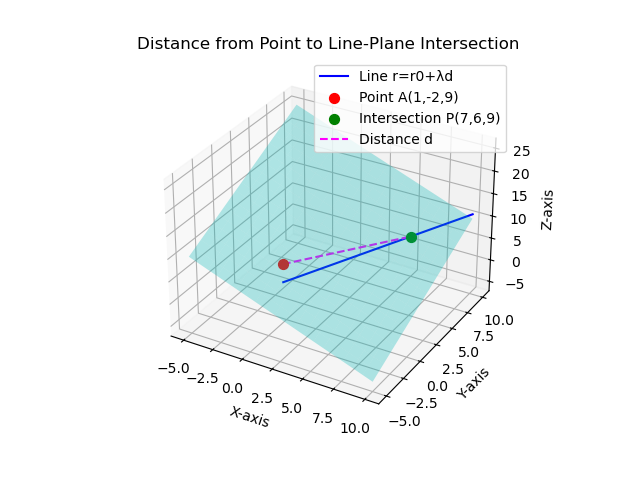
\includegraphics[width=0.7\columnwidth]{figs/Figure_1.png}
    \caption{Intersection point $P$, given point $A$, and distance $AP$.}
    \label{fig:fig1}
\end{figure}

\end{document}













